\documentclass[border=3mm]{standalone}
\usepackage{pgfplots}\pgfplotsset{compat=1.18}
\usepackage{fontspec}\setmainfont{Liberation Sans}
\usepackage{unicode-math}\setmathfont{TeX Gyre DejaVu Math}\newcommand{\Ohm}{Ω}
\usetikzlibrary{arrows.meta}
\definecolor{dunkel}{HTML}{1F3A5F}\definecolor{heiss}{HTML}{E4572E}\definecolor{gruen}{HTML}{2E7D4F}\definecolor{grau}{HTML}{6B6B6B}
\begin{document}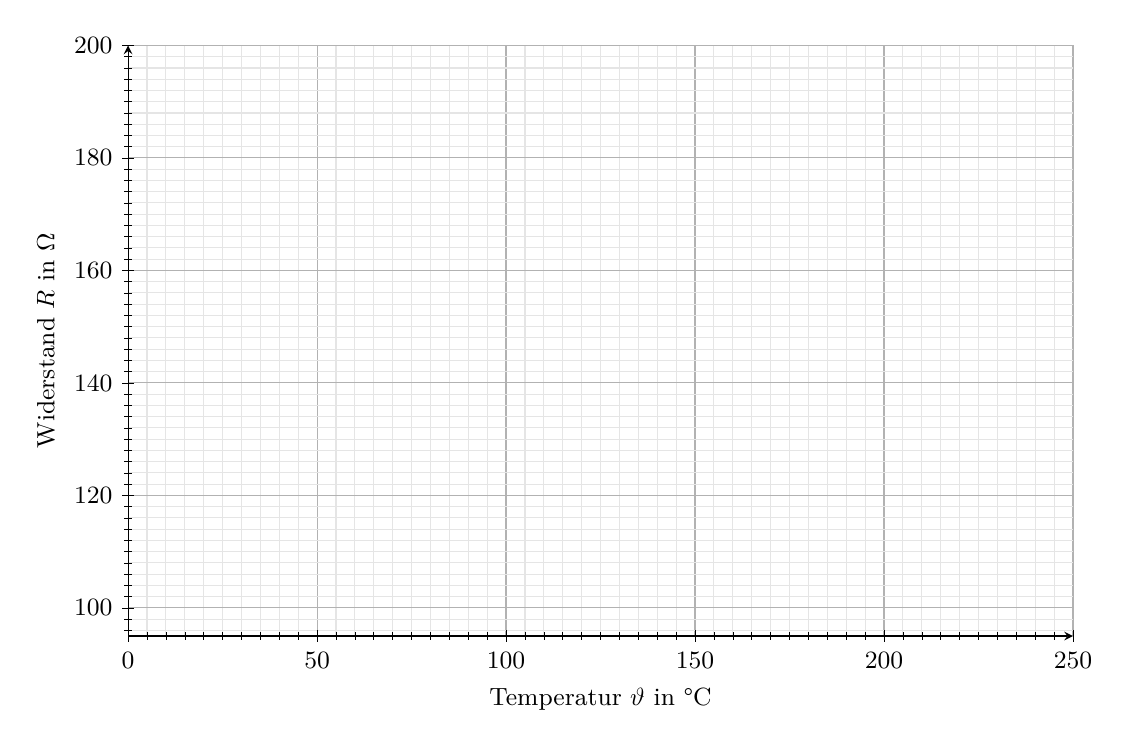
\begin{tikzpicture}
\begin{axis}[width=12cm,height=7.5cm,scale only axis,xmin=0,xmax=250,ymin=95,ymax=200,xlabel={Temperatur $ϑ$ in °C},ylabel={Widerstand $R$ in \Ohm{}},grid=both,grid style={black!15},minor tick num=4,minor grid style={black!6},axis lines=left,tick style={black},/pgf/number format/use comma,/pgf/number format/1000 sep={\,},every axis label/.style={font=\small},tick label style={font=\small},legend cell align=left,xticklabel={\pgfmathprintnumber[assume math mode=true]{\tick}},yticklabel={\pgfmathprintnumber[assume math mode=true]{\tick}},legend style={draw=none,fill=white,font=\footnotesize,at={(0.02,0.98)},anchor=north west},xtick distance=50,ytick distance=20,minor tick num=9,minor grid style={black!10},grid style={black!30}]

\end{axis}
\end{tikzpicture}\end{document}
